\subsection{Fluid-Structure Interaction between an elastic object and laminar incompressible flow} \label{sec:HronTurek}
The benchmark used in this chapter is called \say{Proposal for numerical benchmarking of fluid-structure interaction between an elastic object and laminar incompressible flow} \cite{Hron2006a}, based on an older well known CFD benchmark\cite{Turek1996}. 
The authors provides a computational domain, and boundary conditions, splitting up into a: computational solid mechanical (CSM) part called CSM1-3, a CFD part called CFD1-3 and a full FSI part named FSI1-3. Providing in total 9 subproblems with 3 problems in each part. The chapter starts by defining the computing domain, the boundary conditions and quantities for comparison. For the sake of completeness we split up into the three parts, CSM, CFD and FSI, listing how the subtests are computed and providing results.

\subsection*{Problem Defintion}
\subsubsection*{Domain}
\begin{center}
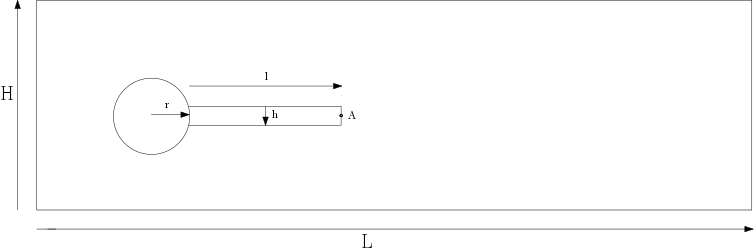
\includegraphics[scale=0.4]{./Verification_Validation/Hron_Turek/Domain_drawing.png}
\end{center}

The computational domain consists of a circle with an elastic bar behind the circle. The circle is positioned at (0.2, 0.2) making it 0.05 off center from bottom to top. This shift in the domain is done to induce oscillations to an otherwise symmetric flow.
\begin{table}[H]
\centering
\caption{Domain parameters}
\label{my-label}
\begin{tabular}{|l|l|l|l|l|}
\hline
L & H & l & h & A \\ \hline
2.5 & 0.41 & 0.35 & 0.02 & (0.2, 0.6) \\ \hline
\end{tabular}
\end{table}

The mesh shown in figures \ref{fig:fullmesh} and \ref{fig:partmesh} were made using Gmsh, with 11556 Cells, which is the mesh with the smallest node spacing. Table \ref{meshes} shows the number of cells and dofs used in each mesh. Elements are the computational cells in the mesh and dofs are the \textit{degrees of freedom}, often called the number of unknowns.

\begin{table}[H]
\centering
\label{meshes}
\begin{tabular}{|l|l|l|}
\hline
Mesh level & Elements & Dofs \\ \hline
1 & 2474 & 21749 \\ \hline
2 & 7307 & 63365 \\ \hline
3 & 11556 & 99810 \\ \hline
\end{tabular}
\caption{Mesh levels showing number og cells and dofs in each mesh}
\end{table}

\begin{figure}[H]
\centering
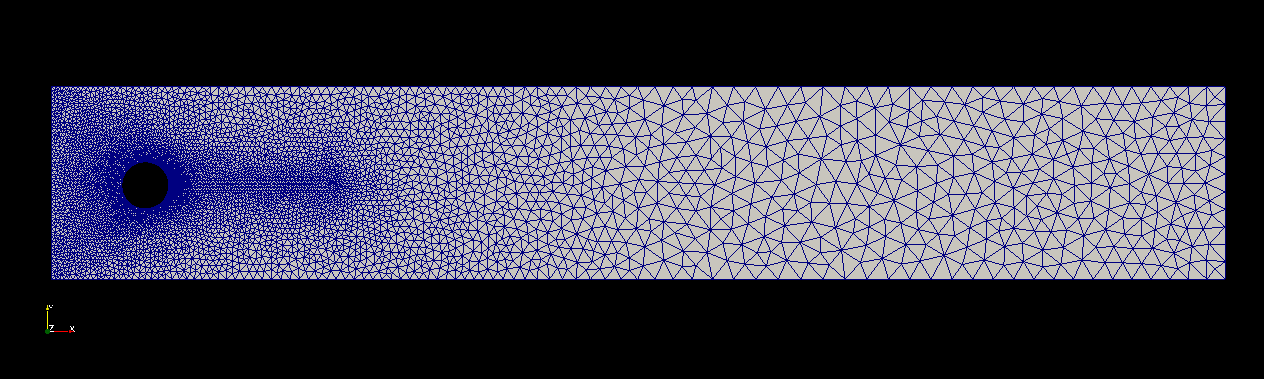
\includegraphics[scale=0.40,trim={20mm 34mm 20mm 30mm},clip]{./Verification_Validation/Hron_Turek/FSI_domain_b2.png}
\caption{Picture of entire FSI computing domain with 11556 cells}
\label{fig:fullmesh}
\end{figure}
\begin{figure}[H]
\centering
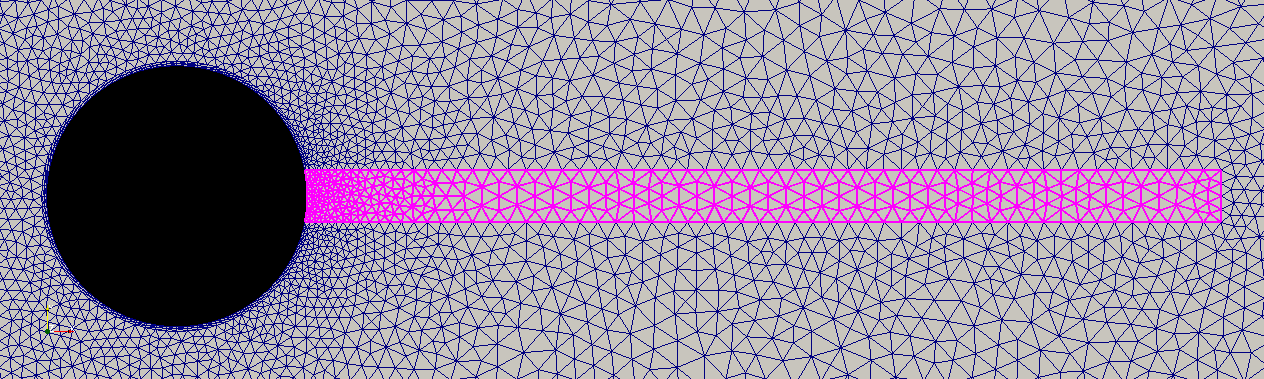
\includegraphics[scale=0.362,trim={0mm 0mm 0mm 0mm},clip]{./Verification_Validation/Hron_Turek/FSI_domain_b2_zoom.png}
\caption{Picture of FSI computing domain with 11556 cells, zoomed in with the solid domain marked in pink. Around the circle we can see a small boundary layer with the width of 2 cells}
\label{fig:partmesh}
\end{figure}



\subsubsection*{Boundary conditions}
A parabolic profile has been prescribed to the inlet velocity that increases from $t=[0,2]$ and is kept constant after $t = 2$.
The fluid velocity on upper and lower walls are set to zero, normally called a \say{no slip} condition.

\begin{align*}
u(0,y) &= 1.5u_0 \frac{y(H-y)}{(\frac{H}{2})^2}  \\
u(0,y,t) &= u(0,y)\frac{1-cos(\frac{\pi}{2}t)}{2} \text{  for  } t<2.0 \\
u(0,y,t) &= u(0,y) \text{  for  } t \leq 2.0
\end{align*}

\subsubsection*{Quantities for comparison}
When the fluid moves around the circle and bar it exerts a frictional force. These forces are split into drag and lift and calculated as follows:
$$ (F_d, F_L) = \int_S \sigma_f n dS $$ 
where S is the part of the circle and bar in contact with the fluid. \\
We set a point $A = (0.2,0.6)$ on the right side of the bar. Where this point is in the spatial direction gives a value for how much the bar has deflected. \\
For some given inflow conditions, unsteady solutions appear. For the unsteady solutions the values, meaning drag and lift, and displacement in x and y directions, are represented by the mean and amplitude values:
\begin{align}
mean =& \frac{1}{2} (max + min) \\
amplitude =& \frac{1}{2} (max - min)\\
\end{align}

In each test the values denoted as \textbf{ref} are the values taken from the original benchmark proposal paper \cite{Hron2006a}. 

\subsubsection{CFD test cases}
The CFD tests can be simulated in two ways. The first way assumes the bar to be rigid object, meaning that the computational domain consists of the fluid domain only, and a no slip condition has been set on the interface. The other way, which is implemented in this thesis, is by computing the problem as a full FSI problem by setting $\rho_s=10^{6}$ and $\mu_s=10^{12}$, such that the bar is almost completely rigid, only giving rise to very small deformation (in the $10^{-9}-10^{-10}$ range).

The CFD tests cases, CFD1 and CFD2 are simulated with Reynolds numbers 20 and 100 converging to steady solutions, \ref{tab:cfd_para}. The CFD3 test case has a Reynolds number 200 which will induce oscillations behind the circle and bar, giving fluctuations in the fluid velocity, hence giving unsteady solutions.

\vspace{1cm}

\begin{table}[H]
\centering
\caption{Summary of all the parameters in CFD tests}
\label{tab:cfd_para}
\begin{tabular}{|l|l|l|l|}
\hline
Parameters & CFD1 & CFD2 & CFD3 \\ \hline
$\rho_f [10^3 \frac{kg}{m^3}]$ & 1 & 1 & 1 \\ \hline
$\nu_f [10^{-3} \frac{m^2}{s}]$ & 1 & 1 & 1 \\ \hline
$ U [\frac{m}{s}] $ & 0.2 & 1 & 2 \\ \hline
Re = $\frac{Ud}{\nu_f}$ & 20 & 100 & 200 \\ \hline
\end{tabular}
\end{table}

\begin{figure}[H]
\label{fig:CFD2}
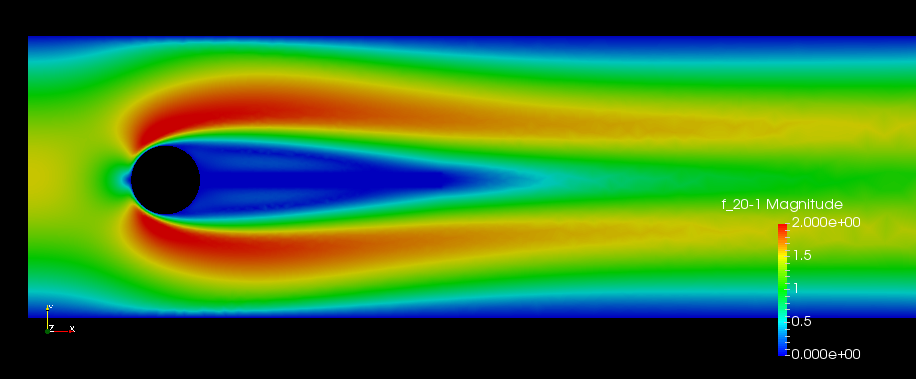
\includegraphics[scale=0.45, trim={9mm 0mm 0mm 10mm},clip]{./Verification_Validation/Hron_Turek/CFD2.png}
\caption{CFD2 steady state case fluid flow with 11556 cells}
\end{figure}

Notice in figure \ref{fig:CFD2}, which shows the fluid flow of the CFD2 case, that since the circle and bar are positioned non symmetric in the y direction there is more fluid flowing closer to the upper boundary. This non symmetry is what induces oscillations when the fluid inlet velocity is higher. The CFD2 case has an inlet velocity just below the point of inducing oscillations.

Table \ref{tab:CFD1} shows the results for the CFD1 testcase, showing convergence towards the referential values in Drag and Lift for increasing elements and dofs.

\begin{table}[H]
\centering
\caption{Results of CFD1 case run as full FSI, with almost rigid bar}
\label{tab:CFD1}
\begin{tabular}{|l|l|l|l|}
\hline
\textbf{elements} & \textbf{dofs} & \textbf{Drag} & \textbf{Lift} \\ \hline
2474 & 21749 & 14.059 & 1.100 \\ \hline
7307 & 63365 & 14.110 & 1.080 \\ \hline
11556 & 99810 & 14.200 & 1.1093 \\ \hline
\textbf{ref} & \textbf{} & \textbf{14.29} & \textbf{1.119} \\ \hline
\end{tabular}
\end{table}

Table \ref{tab:CFD2} shows the results for CFD2 tending towards the referential values in Drag and Lift for increasing elements and dofs.

\begin{table}[H]
\centering
\caption{Results of CFD2 case run as full FSI with almost rigid bar}
\label{tab:CFD2}
\begin{tabular}{|l|l|l|l|}
\hline
\textbf{elements} & \textbf{dofs} & \textbf{Drag} & \textbf{Lift} \\ \hline
2474 & 21749 & 134.9 & 10.38 \\ \hline
7307 & 63365 & 135.4 & 10.0 \\ \hline
11556 & 99810 & 136.1 & 10.41 \\ \hline
\textbf{ref} & \textbf{} & \textbf{136.7} & \textbf{10.53} \\ \hline
\end{tabular}
\end{table}

Table \ref{CFD3_dt001} shows the results for the CFD3 testcase with $\Delta t = 0.01$, the results show clear convergence toward the \textbf{ref} value for increased number of cells and dofs.

\begin{table}[H]
\centering
\label{CFD3_dt001}
\begin{tabular}{|l|l|l|l|}
\hline
\textbf{elements} & \textbf{dofs} & \textbf{Drag} & \textbf{Lift} \\ \hline
2474 & 21749 & $434.42 \pm 4.28$ & $-15.63 \pm 407.59$ \\ \hline
7307 & 63365 & $435.54 \pm 5.06$ & $-11.77 \pm 425.73$ \\ \hline
11556 & 99810 & $438.13 \pm 5.42$ & $ -10.01 \pm 435.40 $ \\ \hline
\textbf{ref} & \textbf{ref} & $\bold{439.45} \pm \bold{5.61 }$ & $\bold{ -11.893} \pm \bold{437.81 }$ \\ \hline
\end{tabular}
\caption{Results of unsteady state case CFD 3 with $\Delta t = 0.01$, where the \textbf{ref} was computed with $\Delta t = 0.005$}
\end{table}

The solutions to the CFD1-3 test cases gives satisfactory results compared to the referential values given in the benchmark paper.

\subsubsection{Computational Structural Mechanical test cases}
The CSM tests are calculated using only the bar as computing domain. A body force $f_s$ is set a gravitational force $g$, which has been kept fixed throughout the CSM tests, changing only the material parameters of the solid. The tests CSM1 and CSM2 gives rise to steady state solutions. The difference between them is a more slender bar. 
The CSM 3 gives unsteady solutions, and since there is no friction the bar should, if energy is preserved hence a correct solution, bounce down and back up infinitely. 

\begin{center}
\begin{figure}[H]
\caption{Picture of the coarsest solid mesh used in the MMS test}
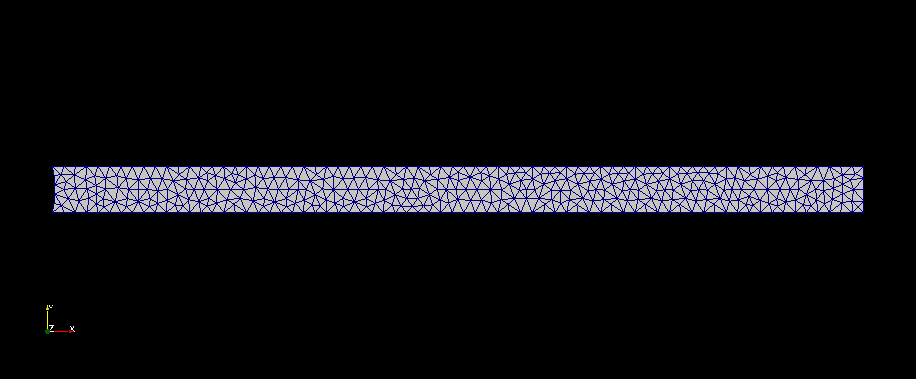
\includegraphics[scale=0.50,trim={18mm 55mm 18mm 55mm},clip]{./Verification_Validation/Hron_Turek/structure.png}
\end{figure}
\end{center}

\vspace{0cm}

\begin{table}[H]
\centering
\caption{Summary table of the parameters used in the CSM tests}
\label{my-label}
\begin{tabular}{|l|l|l|l|}
\hline
Parameters & CSM1 & CSM2 & CSM3 \\ \hline
$\rho_f[10^3 \frac{kg}{m^3}]$ & 1 & 1 & 1 \\ \hline
$\nu_f [10^{-3} \frac{m^2}{s}]$ & 1 & 1 & 1 \\ \hline
$u_0$ & 0 & 0 & 0 \\ \hline
$\rho_s[10^3 \frac{kg}{m^3}]$ & 1 & 1 & 1 \\ \hline
$\nu_s$ & 0.4 & 0.4 & 0.4 \\ \hline
$\mu_s[10^6 \frac{m^2}{s}]$ & 0.5 & 2.0 & 0.5 \\ \hline
$g $ & 2 & 2 & 2 \\ \hline
\end{tabular}
\end{table}

The tables \ref{tab:CSM1} ,\ref{tab:CSM2} and \ref{tab:CSM2} shows the results of the CSM1, CSM2 and CSM3 cases respectively. All three show a clear tendency towards the referential values when increasing the number of elements, and gives satisfactory results.

\begin{table}[H]
\centering
\caption{Results of the steady CSM1 case from coarse to fine mesh.}
\label{tab:CSM1}
\begin{tabular}{|l|l|l|l|}
\hline
elements & dofs & $d_x(A) [\times10^{-3}]$ & $d_y(A) [\times10^{-3}]$ \\ \hline
725 & 1756 & -5.809 & -59.47 \\ \hline
2900 & 6408 & -6.779 & -64.21 \\ \hline
11600 & 24412 & -7.085 & -65.63 \\ \hline
46400 & 95220 & -7.116 & -65.74 \\ \hline
\textbf{ref} & \textbf{ref} & \textbf{-7.187} &  \textbf{-66.10} \\ \hline
\end{tabular}
\end{table}

\begin{table}[H]
\centering
\caption{Results of the steady CSM2 case from coarse to fine mesh.}
\label{tab:CSM2}
\begin{tabular}{@{}|l|l|l|l|@{}}
\hline
Elements & Dofs & $d_x(A) [\times10^{-3}] $& $d_y(A) [\times10^{-3}] $\\ \hline
725 &  1756 & -0.375 & -15.19 \\ \hline
2900 & 6408 & -0.441 & -16.46\\ \hline
11600 & 24412 & -0.462 & -16.84 \\ \hline
46400 & 95220 & -0.464 & -16.87\\ \hline
\textbf{ref} & \textbf{ref} &  \textbf{-0.469} &  \textbf{-16.97} \\ \hline
\end{tabular}
\end{table}

\begin{table}[H]
\centering
\caption{Results of the unsteady CSM3 case with mesh from coarse to fine.}
\label{tab:CSM3}
\begin{tabular}{|l|l|l|l|}
\hline
elements & dofs & $d_x(A) [\times10^{-3}]$ & $d_y(A)[\times10^{-3}]$ \\ \hline
725 & 1756 & $-11.743 \pm 11.744$ & $-57.952 \pm 58.940$ \\ \hline
2900 & 6408 & $-13.558 \pm 13.559$ & $ -61.968 \pm  63.440 $ \\ \hline
11600 & 24412 & $ -14.128 \pm 14.127$ & $-63.216 \pm 64.744 $ \\ \hline
46400 & 95220 & $ -14.182 \pm 14.181 $ & $ -63.305 \pm 64.843 $ \\ \hline
\textbf{ref} &  & $ \textbf{-14.305} \pm \textbf{14.305} $ & $ \textbf{-63.607} \pm  \textbf{65.160} $ \\ \hline
\end{tabular}
\end{table}

The figure \ref{plot:CSM3} is of displacement at the point A in x and y direction of the CSM3 test. The CSM3 test was run with Crank-Nicholson, $\theta = 0.5$, and it can be seen that in the y displacement the bar returns to it initial state, that is with zero displacement. This results indicates that the energy in the system has been preserved.

\begin{figure}[H]  
\centering
  \begin{minipage}[b]{0.60\linewidth}
    \centering
    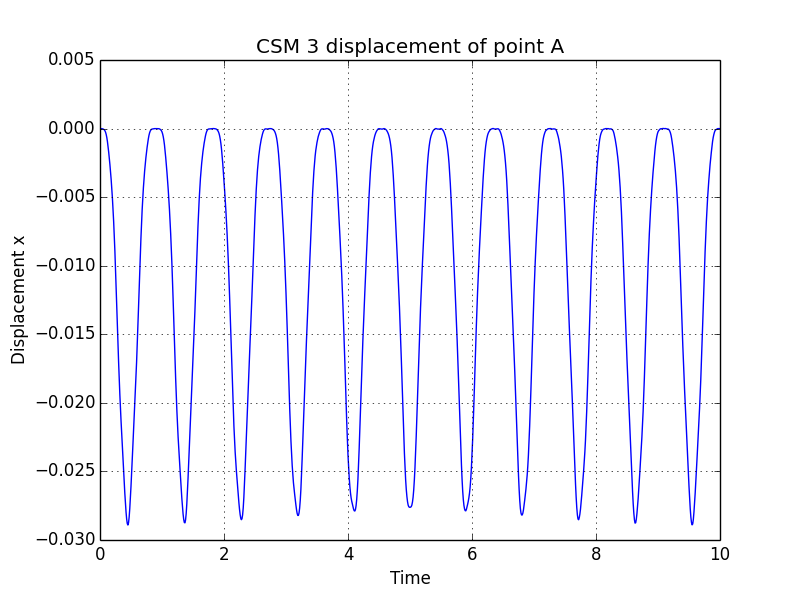
\includegraphics[width=0.9\linewidth,trim={2mm 2mm 5mm 5mm},clip]{./Verification_Validation//Hron_Turek/dis_x.png} 
    \caption{Displacement in x direction, timeinterval (0,10)} 
    \vspace{4ex}
  \end{minipage}%%
  \begin{minipage}[b]{0.60\linewidth}
    \centering
    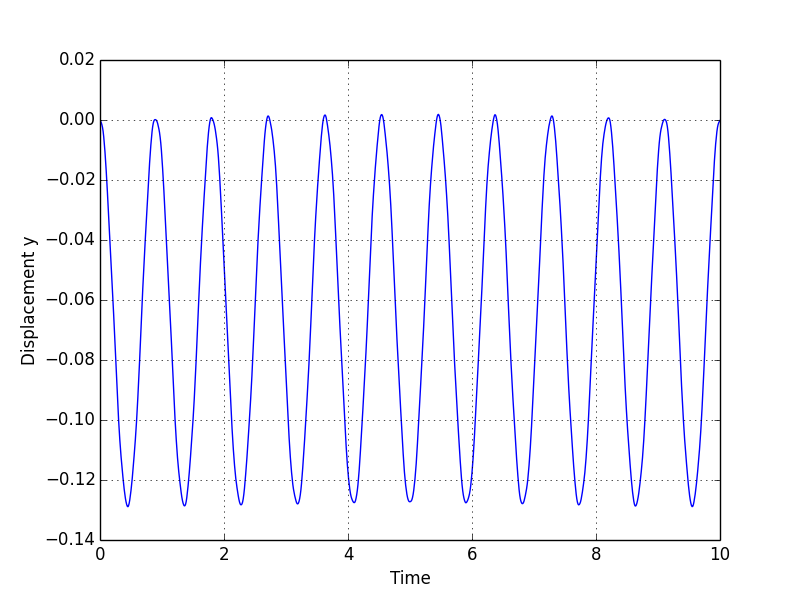
\includegraphics[width=0.9\linewidth,trim={2mm 2mm 5mm 5mm},clip]{./Verification_Validation//Hron_Turek/dis_y.png} 
    \caption{Displacement in y direction, timeinterval (0,10)} 
    \vspace{4ex}
  \end{minipage} 
  \begin{minipage}[b]{0.60\linewidth}
    \centering
    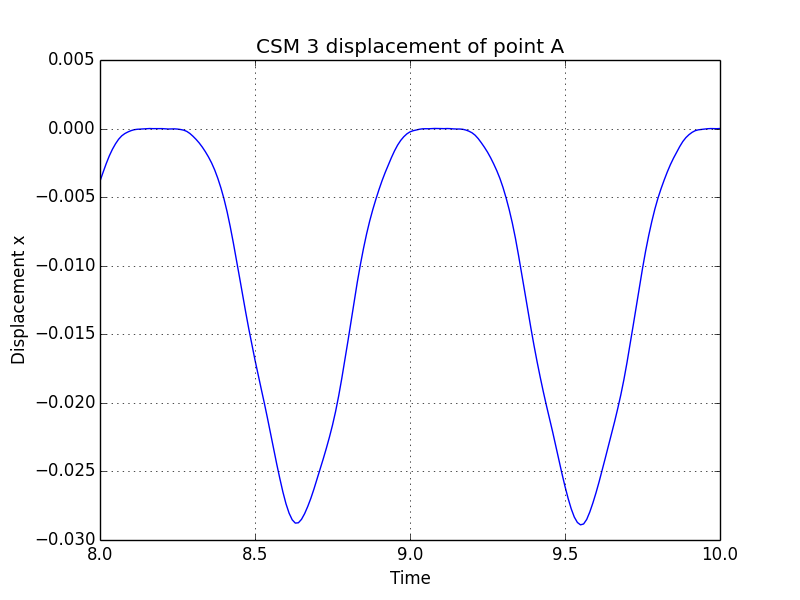
\includegraphics[width=0.9\linewidth,trim={2mm 2mm 5mm 5mm},clip]{./Verification_Validation//Hron_Turek/dis_x_short.png} 
    \caption{Displacement in x direction, timeinterval (8,10)} 
    \vspace{4ex}
  \end{minipage}%% 
  \begin{minipage}[b]{0.60\linewidth}
    \centering
    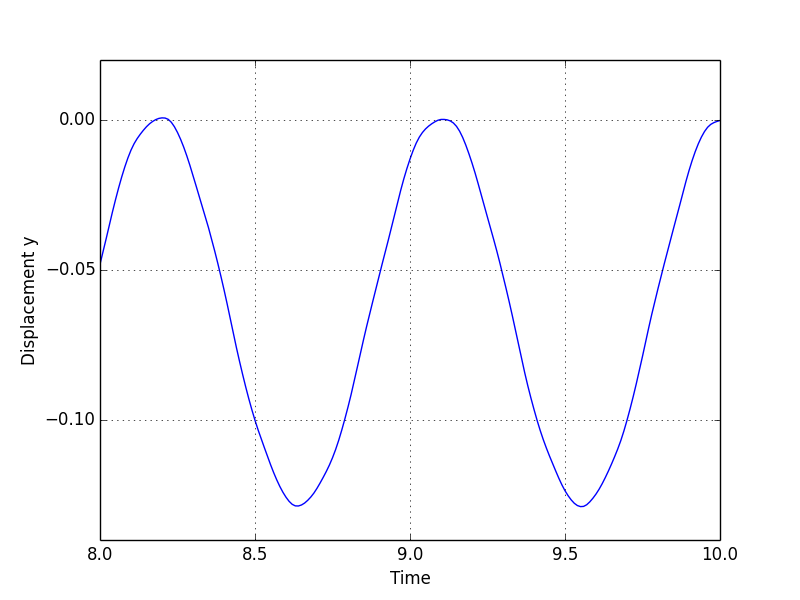
\includegraphics[width=0.9\linewidth,trim={2mm 2mm 5mm 5mm},clip]{./Verification_Validation/Hron_Turek/dis_y_short.png} 
    \caption{Displacement in y direction, timeinterval (8,10)} 
    \vspace{4ex}
  \end{minipage} 
  \caption{Plots of the results for CSM3 showing Displacement of point A}
  \label{plot:CSM3} 
\end{figure}


\subsubsection*{FSI tests}
The FSI tests are run with 2 different inflows conditions. FSI1 gives a steady state solution while the others are unsteady. FSI-2 gives the largest deformation is therefore considered the most difficult of the three \cite{Richter2013}, giving deformations of 2.5 times greater than the flag height. The FSI-3 test has the highest inflow speed giving medium deformations but more rapid oscillations. The parameters for FSI1-3 are shown in table


\begin{table}[h!]
\centering
\caption{FSI Parameters}
\label{my-label}
\begin{tabular}{|l|l|l|l|}
\hline
Parameters & FSI1 & FSI2 & FSI3 \\ \hline
$\rho_f[10^3 \frac{kg}{m^3}]$ & 1 & 1 & 1 \\ \hline
$\nu_f [10^{-3} \frac{m^2}{s}]$ & 1 & 1 & 1 \\ \hline
$u_0$ & 0.2 & 1 & 2 \\ \hline
Re = $\frac{U d}{\nu_f}$ & 20 & 100 & 200 \\ \hline
$\rho_s[10^3 \frac{kg}{m^3}]$ & 1 & 10 & 1 \\ \hline
$\nu_s$ & 0.4 & 0.4 & 0.4 \\ \hline
$\mu_s[10^6 \frac{m^2}{s}]$ & 0.5 & 0.5 & 2 \\ \hline
\end{tabular}
\end{table}

\begin{table}[H]
\centering
\caption{Results of FSI 1 test case}
\label{my-label}
\begin{tabular}{|l|l|l|l|l|l|}
\hline
Cells & Dofs & $d_x(A) [\times10^{-3}]$ & $d_y(A)[\times10^{-3}]$ & Drag & Lift \\ \hline
2474 & 21749 & 0.0229 & 0.8265 & 14.0581 & 0.7546 \\ \hline
7307 & 63365 & 0.02309 & 0.7797 & 14.1077 & 0.7518 \\ \hline
11556 & 99810 & 0.02295 & 0.8249 & 14.2046 & 0.7613 \\ \hline
\textbf{ref} & \textbf{ref} & \textbf{0.0227} & \textbf{0.8209} & \textbf{14.295} & \textbf{0.7638} \\ \hline
\end{tabular}
\end{table}

\begin{figure}[H]
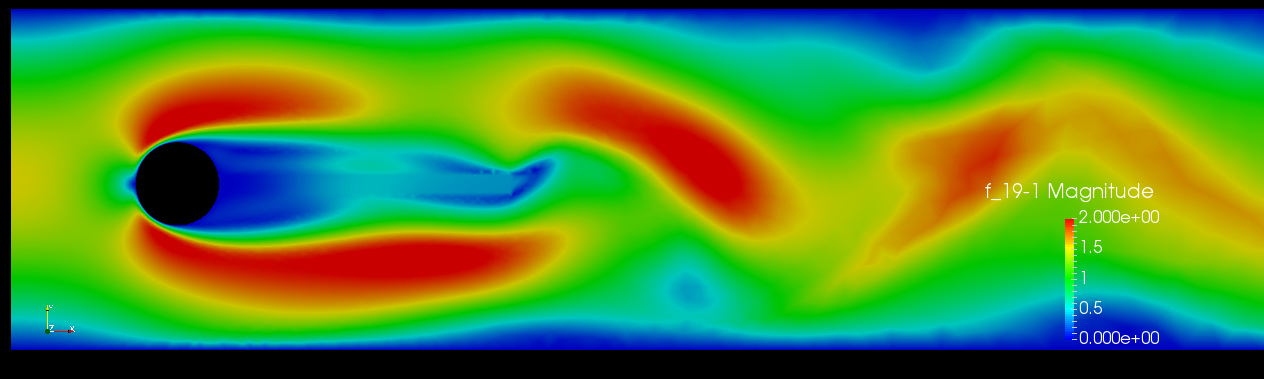
\includegraphics[scale=0.35,trim={0mm 0mm 0mm 0mm},clip]{./Verification_Validation/Hron_Turek/FSI2_u_970.png}
\caption{FSI2 test case Fluid velocity at $ t = 9.70 $sec on the reference mesh}
\end{figure}

\begin{figure}[H]
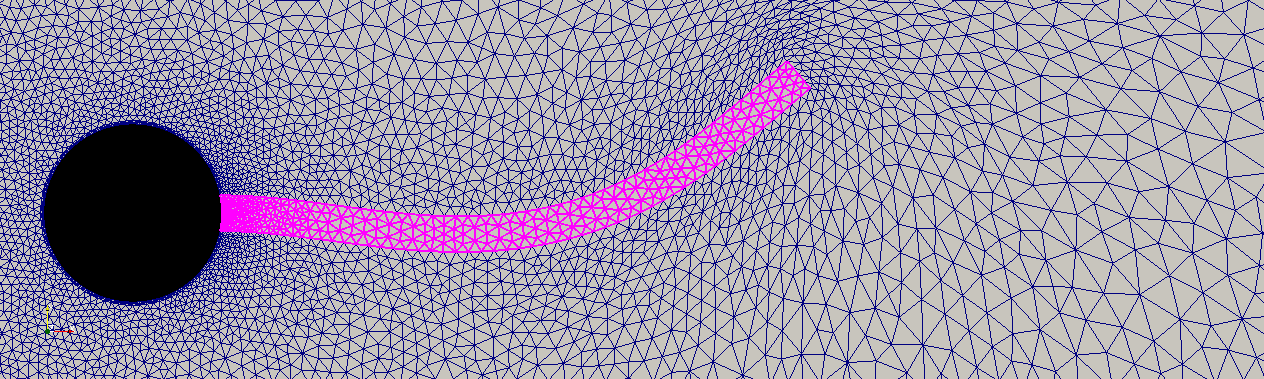
\includegraphics[scale=0.35,trim={0mm 0mm 0mm 0mm},clip]{./Verification_Validation/Hron_Turek/FSI2_d_970.png}
\caption{FSI2 test case deformation at $t =9.70 $sec. The bar is marked with pink colour and deformed using warp by vector in paraview.}
\end{figure}

The tables \ref{FSI2_table} and \ref{FSI2_table_0001} shows results for the FSI2 test case. The displacements in both results for both of the $\Delta t =0.01$ and $\Delta t = 0.001$ show convergence towards the \textbf{ref} values. The lift converges more slowly towards the ref value, while the drag values are off by about a value of 45 in both cases.

\begin{table}[H]
\centering
\caption{FSI2 test case results, $\Delta t = 0.01$, using the harmonic lifting operator}
\label{FSI2_table}
\begin{tabular}{|l|l|l|l|l|l|}
\hline
Cells & Dofs & $d_x(A) [\times10^{-3}]$ & $d_y(A) [\times10^{-3}]$ & Drag & Lift \\ \hline
2474 & 21749 & $-15.26 \pm 13.44$ & $1.34 \pm 82.38$ & $157.02 \pm 14.79 $ & $-1.426 \pm 258.4 $ \\ \hline
7307 & 63365 & $-14.96 \pm 13.24$ & $1.01 \pm 81.67$ & $159.01 \pm 16.33$ & $1.88 \pm 254.2 $ \\ \hline
11556 & 99810 & $-14.96 \pm 13.23 $ & $1.29 \pm 81.9 $ & $ 161.09 \pm 17.66 $ & $0.06 \pm 255.78 $ \\ \hline
\textbf{ref} & \textbf{ref} & $\textbf{-14.58} \pm \textbf{12.44}$ & $\textbf{1.23} \pm \textbf{80.6}$ & $\textbf{208.83} \pm \textbf{73.75}  $ & $\textbf{0.88} \pm \textbf{234.2} $ \\ \hline
\end{tabular}
\end{table}

\begin{table}[H]
\centering
\caption{FSI-2 with $\Delta t = 0.001$, using harmonic lifting operator}
\label{FSI2_table_0001}
\begin{tabular}{|l|l|l|l|l|l|}
\hline
Cells & Dofs & $d_x(A) [x10^{-3}]$ & $d_y(A) [x10^{-3}]$ & Drag & Lift \\ \hline
2474 & 21749 & $ -15.10 \pm 13.32 $ & $1.16 \pm 82.46 $ & $ 159.53 \pm 17.44 $ & $ 0.68 \pm 259.10 $ \\ \hline
7307 & 63365 & $ -14.85 \pm 13.14 $ & $1.21 \pm 81.72 $ & $ 160.72 \pm 17.84  $ & $0.93 \pm 255.14 $ \\ \hline
11556 & 99810 & $ -14.83  \pm 13.11  $ & $ 1.24 \pm 81.6 $ & $ 161.50 \pm 18.17  $ & $0.62 \pm 254.40  $ \\ \hline
\textbf{ref} & \textbf{ref} & $\textbf{-14.58} \pm \textbf{12.44}$ & $\textbf{1.23} \pm \textbf{80.6}$ & $\textbf{208.83} \pm \textbf{73.75}  $ & $\textbf{0.88} \pm \textbf{234.2} $ \\ \hline
\end{tabular}
\end{table}

\begin{figure}[H] 
  \label{FSI2_plots} 
  \begin{minipage}[b]{0.6\linewidth}
    \centering
    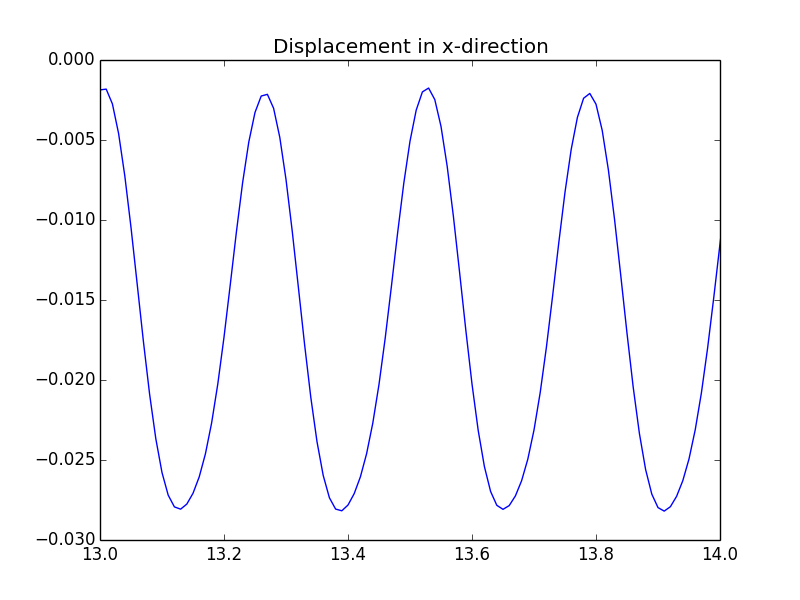
\includegraphics[width=0.9\linewidth]{./Verification_Validation/Hron_Turek/FSI2_dis_x.png} 
    \caption{Displacement x} 
    \vspace{4ex}
  \end{minipage}%%
  \begin{minipage}[b]{0.6\linewidth}
    \centering
    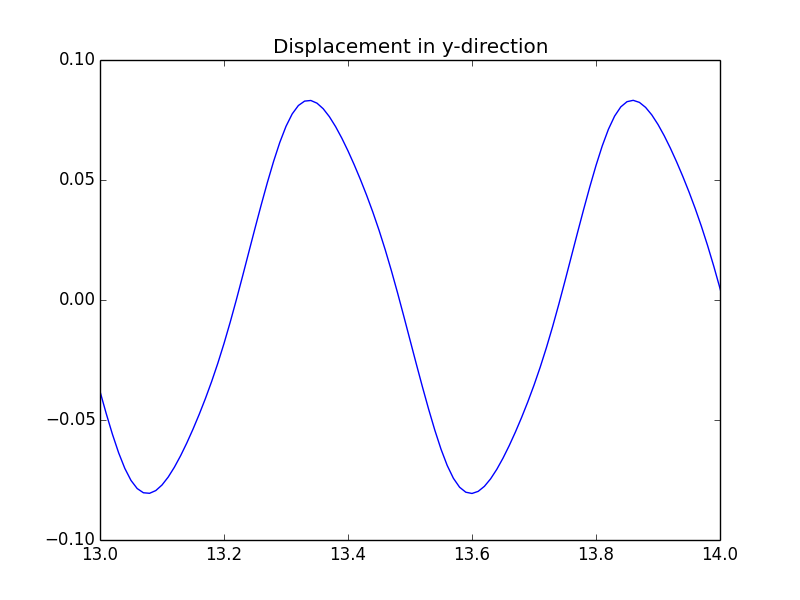
\includegraphics[width=0.9\linewidth]{./Verification_Validation/Hron_Turek/FSI2_dis_y.png} 
    \caption{Displacement x} 
    \vspace{4ex}
  \end{minipage} 
  \begin{minipage}[b]{0.6\linewidth}
    \centering
    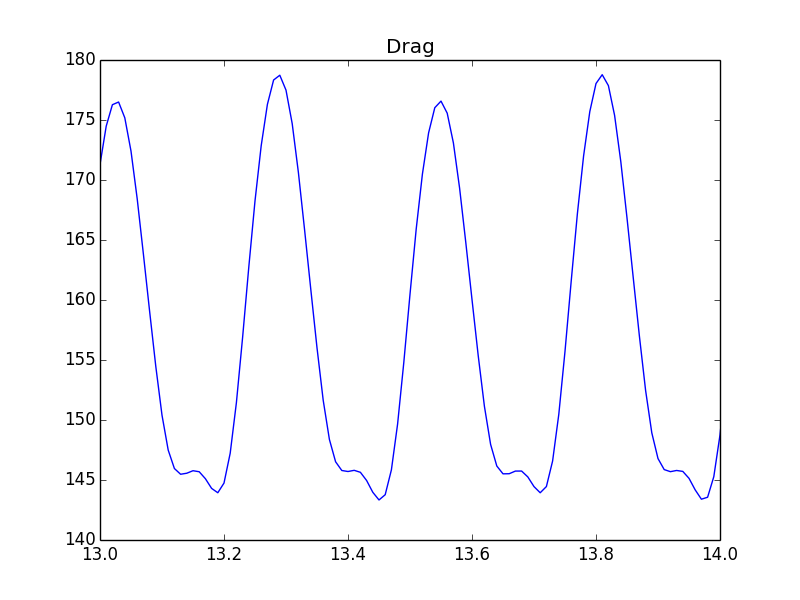
\includegraphics[width=0.9\linewidth]{./Verification_Validation/Hron_Turek/FSI2_drag.png} 
    \caption{Drag} 
    \vspace{4ex}
  \end{minipage}%% 
  \begin{minipage}[b]{0.6\linewidth}
    \centering
    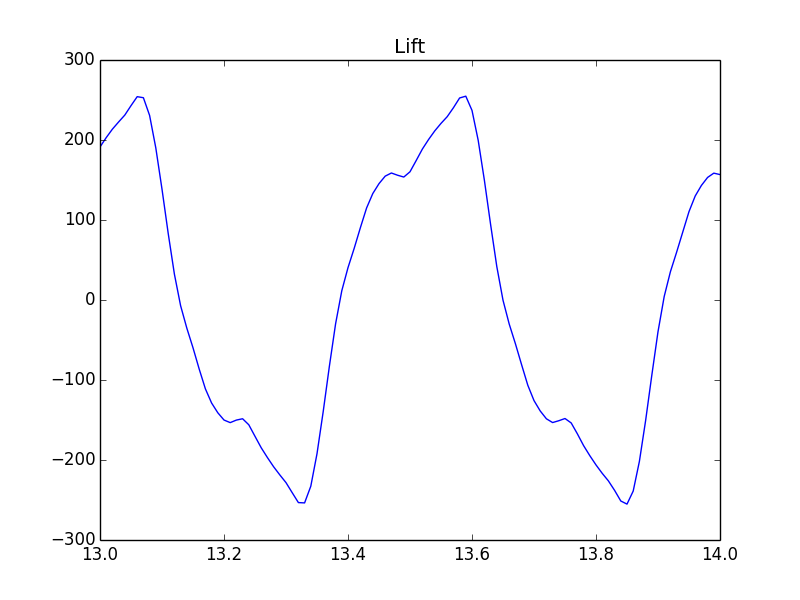
\includegraphics[width=0.9\linewidth]{./Verification_Validation/Hron_Turek/FSI2_lift.png} 
    \caption{Lift} 
    \vspace{4ex}
  \end{minipage} 
  \caption{Plots of FSI2 result values for, $\Delta t = 0.001$, with 11556 elements}
\end{figure}

In tables \ref{tab:FSI3_001} and \ref{tab:FSI3_0001} shows that results for FSI3 with $\Delta t = 0.01$ and $\Delta t = 0.001$, respectively. Both tables show convergence for displacements in both directions and for drag. In the results for lift the values are more scattered and not showing a clear trend but still within 50 \% of the referential values.

\begin{table}[H]
\centering
\caption{FSI3 unsteady test case results with $\Delta t = 0.01$, with biharmonic bc1 lifting operator}
\label{tab:FSI3_001}
\begin{tabular}{|l|l|l|l|l|l|}
\hline
Cells & Dofs & $d_x (A)[\times10^{-3} ]$ & $d_y (A)[\times10^{-3} ]$ & Drag & Lift \\ \hline
2474 & 21249 & $-1.79 \pm 1.80$ & $3.29 \pm 2.64$ & $439.36 \pm 12.04$ & $1.96 \pm 142.31$ \\ \hline
7307 & 63365 & $-2.48 \pm 2.48$ & $ 1.64 \pm 3.28$ & $449.77 \pm 18.02$ & $3.41 \pm 153.47$ \\ \hline
11556 & 99810 & $ -2.47 \pm 2.45$ & $ 1.27 \pm 3.28$ & $456.60 \pm 18.73$ & $1.55 \pm 153.46$ \\ \hline
ref & ref & $\bold{-2.69 \pm  2.56}$ & $\bold{1.48 \pm 34.38}$ & $\bold{457.3 \pm 22.66}$ & $\bold{2.22 \pm 149.78}$ \\ \hline
\end{tabular}
\end{table}

\begin{table}[H]
\centering
\caption{FSI3 unsteady test case results with $\Delta t = 0.001$, with biharmonic bc1 lifting operator}
\label{tab:FSI3_0001}
\begin{tabular}{|l|l|l|l|l|l|}
\hline
Cells & Dofs & $d_x (A)[\times10^{-3} ]$ & $d_y (A)[\times10^{-3} ]$ & Drag & Lift \\ \hline
2474 & 21249 & $ -2.188 \pm 2.11 $ & $ 3.56 \pm 2.90 $ & $ 435.19 \pm 9.77$ & $ -1.57 \pm 151.43 $ \\ \hline
7307 & 63365 & $ -1.42 \pm 4.70 $ & $ 0.77 \pm 28.50 $ & $ 454.38 \pm 19.75 $ & $1.79 \pm 155.08 $ \\ \hline
11556 & 99810 & $ -2.23 \pm 6.164 $ & $ 1.72 \pm 4.48 $ & $ 459.12 \pm 22.97 $ & $ 3.12 \pm 171.22 $ \\ \hline
\textbf{ref} & \textbf{ref} & $\bold{-2.69} \pm \bold{2.56}$ & $\bold{1.48} \pm \bold{34.38}$ & $\bold{457.3} \pm \bold{22.66}$ & $\bold{2.22} \pm \bold{149.78}$ \\ \hline
\end{tabular}
\end{table}

\subsection*{Comment on FSI tests}
 A very important thing to notice about this benchmark \cite{Hron2006a} is that it is a proposal for a benchmark, as it is called \say{Proposal for numerical benchmarking of fluid-structure interaction between an elastic object and laminar incompressible flow}. So the point of the paper is give a specific problem setup which others can contribute result-data. A paper was published in 2010 by J. Hron, Turek, et al, \cite{Turek2010} that compared results of different discretizations and solution approaches. This paper \cite{Turek2010} gives 7 different methods and results for two of the FSI test cases. They state in the numerical results that \say{However, also clear differences between the different approaches with regard to accuracy are visible. Particularly for the drag and lift values, which lead to differences of up to order 50\%, and also for the displacement valueswhich are in the range of 10\% errors.}. With this in mind it is important to know that the referential values used are only those reported from the original paper, which only looked at one implementation. While the paper which compares results, only 2 of the 7 contributions were schemes of monolithic nature, which are the closest one should refer to in this thessis.  In the Appendix \ref{sec:bigboys} is a copy of the results from the paper comparing schemes, showing different results for different discretization, with different time steps and unknowns. 

The FSI1 test gives a low fluid velocity and gives very low displacements. FSI1 is therefore not a rigid test for FSI. In fact I personally experienced in the beginning of making the FSI solver, that even with a wrong implementation I got good FSI1 results. However it is a good test for early checks, because if FSI1 is wrong the rest will definitely not work.  \newline

For the FSI2 test case we only have results from the initial Hron and Turek paper \cite{Hron2006a}. As previously stated the results for the FSI3 case differ by in some cases 50\% for Drag and Lift. With this in mind, in the FSI2 case I am off by less then 10\% for displacement in x and y direction and for Lift. While Drag is off by about  50\%. It is reasonable to assume that since there were such differences in the results for different implementations for the FSI3 results, we would expect similar behavior in the FSI2 results.

If we compare the results reported in the FSI3 case in the inital paper by Hron and Turek 2006, to their reported results in 2010 \ref{sec:bigboys} implementation 3, we can see that they do not report the same results same scheme, leading one believe that that they have changed their implementation a bit. 

A note should be added about the construction of the computational meshes. If we look at figures \ref{fig:fullmesh} and \ref{fig:partmesh}. The node spacing on the inlet is small to ensure that the parabolic inlet profile is upheld. There is also smaller node spacing around the circle and around the bar, leading to larger node spacing as we move down stream. In the unsteady CFD and FSI cases there is vortex shedding happening downstream. With large node spacing in this area the vortexes may not be produced to its full extent, hence introducing errors in the unsteady results. 

In hindsight, larger gaps in the number of elements between each mesh should have been larger. The three meshes that are mainly used go from 2474 cells to 7307 cells to 11556 cells. When calculating in 2D to see converging effects in the results of smaller node spacing, one should make meshes with 4 times the number of cells for each new mesh. This might have helped in converging to the referential values. The reason for not being able to run lower values for $\Delta t$ or increased number of cells in the meshes was a lack of computational resources.

\begin{comment}
FSI2 has a Reynolds number of 100 with medium fluid speeds. It does however induce great deformations and is therefore a great FSI test. Using a mesh motion technique that upholds the mesh structure is crucial. The results shown are with the Harmonic extension but I got similar results for biharmonic extension. The FSI2 test could be run with a fairly large time $\Delta t = 0.01 $, since the fluid velocity is not very high. And it can been seen from the results that choosing a time step $\Delta t = 0.001$ did not yield much better results. The Drag was computed to be about a value of 40 less than reported by Hron and Turek. This i believe is because a combination of the way the mesh was constructed, without a good enough boundary layer, and the mapping to a reference configuration. +++ \newline

Lastly the FSI3 test has a Reynolds number of 200 with greater inflow speeds. The run time improvements such as reusing the jacobian did not work with the FSI3 test. The Jacobian needed to be more precise than for FSI2. For this reason a different mesh, with lower number of cells needed to be used in FSI3.  +++
\end{comment}
















